\chapter{Implementacion}
 
 Para explicar la implementación realizada se van a incluir pequeños fragmento del código de los archivos escritos para la aplicación. Estos fragmentos solo contendrán las líneas más significativas, que además irán acompañados de una descripción sobre su significado y funcionamiento.
 
\section{Uso de JSON como origen de datos}
 
Inicialmente el origen de datos para las tablas de las páginas del portal de transparencia era una base de datos \textit{NoSQL} montada sobre un sistema {\tt MongoDB}. Aunque inicialmente funcionaba, había problemas relacionados con el funcionamiento asíncrono de {\tt Node.js}; por dicho funcionamiento \textit{asíncrono} el proceso de generar la página del portal y el proceso de acceder a la información de la base de datos eran independientes en su ejecución aunque dependientes en su funcionamiento, por lo que a no ser que ambos procesos estuvieran perfectamente sincronizados esto derivaría en la aparición de problemas.

\bigskip
Como no se consiguió que se sincronizaran los \textit{callbacks} de ambos procesos eventualmente se producía uno de las situaciones cuando se intentaba cargar una página:

\begin{itemize}
	\item Si la página se intentaba cargar antes de que se hubiera podido acceder a la base de datos, las tablas con datos a visualizar no existían, por lo que se producía un error interno con el código 500.
	\item Si la página se intentaba cargar antes de que se hubieran podido recuperar todos los datos de la base de datos las tablas de datos se generaban vacías, por lo que las páginas que se cargaban se cargaban en blanco.
	\item Solo si la llamada a la base de datos se resolvía antes de que se intentara mostrar la información, la página se mostraba correctamente. 
\end{itemize}

Después de replantear la situación, se consideró que como todos los datos iban a estar finalmente almacenados en la plataforma {\tt OpenData UGR}, la solución más recomendable era eliminar la base de datos y usar en su lugar archivos \textit{JSON} que hicieran de índices de enlaces hacía los conjuntos de datos {\tt OpenData UGR} desde el portal de transparencia. La ventaja de usar archivos \textit{JSON} es la gran flexibilidad que proporcionan a la hora de realizar estructuras de datos; aprovechando esto se diseñaron estos archivos con los siguientes campos (ejemplo en el \textit{fragmento de código 6.1}):

\begin{itemize}
	\item \textbf{nombre}: es la subcategoría en el portal de transparencia.
	\item \textbf{plantilla}: el archivo de plantilla a partir del que se generan las páginas del portal de transparencia.
	\item \textbf{cotenido}: conjunto con la información de cada una de las tablas que muestran en las páginas del portal de transparencia.
	\begin{itemize}
		\item \textbf{encabezado}: nombre de la tabla.
		\item \textbf{link}: salto a la posición de la página donde empieza la tabla.
		\item \textbf{texto}: descripción de los datos que contiene la tabla.
	\end{itemize}
	\item datos: conjunto con los elementos que componen cada una de las tablas.
	\begin{itemize}
		\item \textbf{dataset}: tabla a la que pertenece el elemento.
		\item \textbf{id\_dataset}: conjunto de datos en {\tt OpenData UGR} al que pertenece el elemento.
		\item \textbf{nombre}: descripción del elemento que visualizará en la tabla.
		\item \textbf{vista}: valor que indica si el elemento se puede previsualizar desde el propio portal de transparencia (en caso de ser 1) o si solo se puede visualizar accediendo a su enlace a {\tt OpenData UGR} (en caso de ser 0).
		\item \textbf{url}: dirección al elemento como recurso dentro de {\tt OpenData UGR} para poder ser visualizado.
		\item \textbf{descarga}: dirección de descarga directa del elemento almacenado como recurso en {\tt OpenData UGR}.
	\end{itemize}
\end{itemize}

\newpage
\begin{lstlisting}[language=json,caption={Archivo JSON con informacion de personal},label={lst:json_personal}]
{
  "nombre":"Personal",
  "plantilla":"personal",
  "contenido":[
    {
      "encabezado":"Informacion Salarial 2015",
      "link":"informacion-salarial-2015",
      "texto":"Informacion relativa a la oferta..."
    },
    
  ],
  "datos":[
    {
      "dataset":"Informacion Salarial 2015",
      "id_dataset":"informacion-salarial-2015",
      "nombre":"Analisis total plantilla: genero",
      "vista":1,
      "url":"51d53138-0408-4257-9909-57acea137a58",
      "descarga":"985a8e1e-734b-432a-ac65-a7da..."
    },
        
  ]
}
\end{lstlisting}

Para que estos archivos puedan ser utilizados desde la aplicación, tenemos que convertir los archivos \textit{JSON} en objetos \textit{JSON}, esto lo podemos hacer fácilmente usando dos sencillos métodos como vemos en el \textit{fragmento de código 6.2}. Ambos métodos pertenecen al módulo {\tt cargar.js} de la carpeta \textbf{lib}:

\begin{itemize}
	\item {\tt readFileSync}: es un método del módulo {\tt Fs} (módulo encargado de realizar las operaciones de entrada/salida en {\tt Node.js}) que nos permite leer de forma síncrona los archivos que reciba como argumento.
	\item {\tt JSON.parse}: es un método del objeto \textit{JSON} que nos permite convertir el texto que reciba como argumento en un objeto \textit{JSON} (siempre que este tenga una formato compatible con \textit{JSON}).
\end{itemize}

Es importante aclarar que en {\tt Node.js} los módulos, independientemente de si son creados por nosotros o no, se importan para se usados dentro de módulo con la palabra clave ``\textit{require}'' y se exportan para ser utilizables por otros módulos con la palabra clave ``\textit{export}''.

\newpage
\begin{lstlisting}[language=javascript,caption={Archivo cargar.js},label={lst:cargarjs}]
var fs = require("fs");
 
var cargar = function (archivo){
  var config = null;

  try{
    config = JSON.parse(fs.readFileSync(archivo));
  }
  catch(e){
    console.log("Error: no existe el archivo " + archivo);
  }

  return config;
};

module.exports = cargar;
\end{lstlisting}

Tenemos toda la información como objetos \textit{JSON}, así que ya podemos hacer uso de ella desde nuestra aplicación. Desde la misma aplicación principal lo primero será importar los módulos que nos van a permitir crear la infraestructura web lógica para nuestro portal, estos son los módulos {\tt Express} y {\tt Http}.

\bigskip
El siguiente paso será importar los módulos de cada una de las secciones del portal; en la línea 4 del \textit{fragmento de código 6.3} podemos ver como ejemplo como importamos el módulo de la sección \textit{Administración} que se correspondería con el archivo {\tt administracion.js} de la carpeta \textbf{routes}, la carpeta en la que se encuentran todos los módulos de cada una de las secciones.

\bigskip
A continuación, como vemos en la línea 6, importamos el módulo que hemos descrito antes para la lectura de archivos \textit{JSON} y procedemos a cargar todos los archivos \textit{JSON} de origen de datos que se encuentran en la carpeta \textbf{config}, que se corresponden con la configuración del servidor del portal y los elementos de información de cada una de las secciones.

\bigskip
Otro de los aspectos esenciales en el código de la aplicación principal es crear las rutas para que las páginas del portal de transparencia sean accesibles desde Internet. En la línea 15 vemos como indicar que la ruta de una página de subsección se vincule con la función del módulo que va a generar esa página, en este caso la página de información de \textit{Personal} ({\tt personal.html}) se corresponde al método {\tt personal} del módulo {\tt administracion.js}.

\newpage

Ya solo nos quedaría crear el servidor. Con la línea 8 creamos una instancia del módulo {\tt Express}, ahora mediante el módulo {\tt Http} creamos el servidor sobre esa instancia e indicamos las opciones de accesibilidad necesarias, en este caso el puerto de escucha del servidor ({\tt port}) y la dirección de acceso al portal ({\tt ip}). Finalmente exportamos el módulo de la aplicación principal para más adelante poder realizarle los test los tests unitarios.

\begin{lstlisting}[language=javascript,caption={Archivo app.js},label={lst:appjs}]
var express = require('express');
var http = require('http');

var administracion = require(__dirname+'/routes/administracion');

var cargar = require(__dirname+'/lib/cargar');

var app = express();

config = cargar(__dirname+'/config/config.json');
module.exports.config = config;

module.exports.personal = cargar(__dirname+'/config/personal.json');

app.get('/personal.html',administracion.personal);

http.createServer(app).listen(app.get('port'), app.get('ip'), function(){
  console.log('Express server listening on ' + app.get('ip') + ':' + app.get('port'));
});

module.exports = app;
\end{lstlisting}

La aplicación principal ya está descrita, así que ahora vamos a pasar a los módulos que van a generar las páginas del portal. La estructura de estos módulos es igual en todos los casos, primero se importa el módulo de la aplicación principal para acceder a los archivos JSON de los datos cargados y seguidamente se exporta la función que va a generar cada una de las páginas de las subsecciones del portal (esta es la misma función a la que se llamaba en la línea 15 de la aplicación principal). Cada una de estas funciones contendrá la llamada a una función {\tt render} que será la encargada de pasarle toda la información a la plantilla {\tt Jade} a partir de la que, finalmente, se generará la página web que será accesible en el portal.

\newpage 

\begin{lstlisting}[language=javascript,caption={Archivo administracion.js},label={lst:adminjs}]
var conf = require('../app');

exports.personal = function(req, res){
  var personal = conf.personal;

  res.render(personal.plantilla, {
    servidor: conf.config.servidor,
    seccion: personal.nombre,
    contenido: personal.contenido,
    datos: personal.datos,
  });
};
\end{lstlisting}

Para arrancar y detener la aplicación se usarán dos scripts del archivo {\\package.json} que nos permitirán ejecutar estás tareas con {\tt NPM}. En el caso del script de arranque es necesario que indiquemos los siguientes parámetros:

\begin{itemize}
	\item  El puerto de escucha del servidor (variable {\tt PORT}). Es el puerto del que el servidor estará escuchando las peticiones, en el \textit{fragmento de código 6.5} se ha especificado el puerto 3000 por ser una configuración local (podría ser cualquier otro puerto libre), pero para que el portal sea accesible públicamente se deberá configurar para el puerto 80.
	\item La dirección a través de la que se accederá al portal (variable {\tt IP}). Al igual que en el caso del puerto, la dirección IP indicada (127.0.0.1) es para acceso local únicamente; para un acceso público sería necesario indicar una dirección IP o una URL que sea accesible desde Internet.
\end{itemize}

Con los parámetros especificados, el servidor comenzará a correr ejecutado mediante el módulo {\tt Forever} que hará que la aplicación se ejecute de forma ininterrumpida al ejecutar {\tt ``npm start''}.

\bigskip
Para detener el servidor no tenemos que indicar nada, simplemente ejecutar el script de parada; este se encargará de buscar todos los procesos abiertos por la aplicación principal y mandarles la señal de terminación. Se ejecuta con {\tt ``npm run-script kill''} por no estar reconocido como uno de los scripts por defecto de {\tt NPM}.

\begin{lstlisting}[language=json,caption={Scripts de inicio y detención},label={lst:ini_para}]
"scripts": {
  "start": "PORT=3000 IP=127.0.0.1 forever start -l /var/log/forever.log -a -o /var/log/out.log -e /var/log/err.log ./app.js",
  "kill": "ps aux | grep 'app.js' | grep -v grep | awk '{print \"sudo kill -9 \" $2}' | sh"
}
\end{lstlisting}

\section{Tests unitarios y de cobertura}

Los tests unitarios que se han implementados cumplen con la función de probar la aplicación siendo evaluada en función de comportamientos deseados. Para ello se usarán los módulos {\tt Should} y {\tt Supertest}, el primero evaluará que los archivos \textit{JSON} tengan todos los elementos necesarios para generar las páginas del portal, mientras que el segundo evaluará que las páginas del portal que se generan sean accesibles sin problemas. Todos los tests se encuentran en el archivo {\tt test.js} del directorio \textbf{test}.

\bigskip
En el caso de los archivos \textit{JSON} los comportamientos que tenemos que comprobar son muy simples:

\begin{itemize}
	\item En el caso de cargar un archivo \textit{JSON} con la función {\tt cargar} del módulo {\tt cargar}. Para comprobar que el archivo se ha cargado correctamente, se verifica que el archivo no sea nulo como se comprueba en la línea 10 del \textit{fragmento de código 6.7}.
	\item Con el archivo ya cargado, ahora comprobamos que tiene cada uno de los campos que necesitamos para generar las páginas web; por ejemplo, en la línea 17 comprobamos que el archivo de configuración tengo el campo \textbf{nombre}.
\end{itemize}

Para comprobar que las páginas son accesibles, realizamos una solicitud de la misma a la que el servidor responderá con un código numérico, si ese código tiene el valor \textbf{200} significará que la petición se ha resuelto correctamente, por lo que significará que la página está accesible. Podemos ver como se hace esto observando las líneas 28 a 36.

\bigskip

Acabamos de describir las comprobaciones que realizan los tests, pero nos falta por explicar como se evalúan dichas comprobaciones, los tests unitarios van a ser ejecutados por {\tt Mocha}. Para {\tt Mocha} la ejecución de las pruebas se divide en dos procesos, una descripción que indica qué está evaluando un test unitario o un conjunto de los mismos y la propia evaluación de un test unitario que nos informa si la aplicación supera el test o no; la descripción se realiza con la orden {\tt describe} mientras que la evaluación se realiza con {\tt it}. Un ejemplo de todo esto se puede ver en el \textit{fragmento de código 6.7}.

\newpage
\begin{lstlisting}[language=javascript,caption={Archivo test.js},label={lst:testjs}]
var should = require("should"),
request = require("supertest");

describe('Test de carga y formato de JSONs', function(){
  describe('Archivo de configuracion', function(){
    var config = cargar(__dirname+"/../config/config.json");

    describe('Carga de archivo', function(){
      it('Cargado', function(){
        config.should.not.be.null;
      });
    });

    describe('Formato de archivo', function(){
      describe('Campos obligatorios', function(){
        it('nombre', function(){
          config.should.have.property("nombre");
        });
      });
    });
    
  });
};

describe('Prueba de acceso', function(){
  _.each(acceso.elemento, function(valor) {
    it(valor.nombre, function(done){
      request(app)
      .get(valor.ruta)
      .expect(200)
      .end(function(err, res){
        if (err){
          throw err;
        }
        done();
      });
    });
  });
});
\end{lstlisting}

Al igual que los scripts de inicio y parada de la aplicación principal, los test se ejecutarán mediante un script de {\tt NPM}. Se ha comentado el uso de {\tt Mocha} para pasar los tests unitarios, pero no se ha comentado nada de los tests de cobertura; esto se debe a que el módulo elegido para realizar los tests de cobertura, {\tt Istanbul}, está integrado con {\tt Mocha} para poder realizar automáticamente los tests de cobertura a los tests unitarios que se ejecuten con este último. Ambos se ejecutarán con {\tt ``npm test''}.

\newpage
\begin{lstlisting}[language=json,caption={Scripts de test},label={lst:test}]
"scripts": {
  "test": "istanbul cover _mocha ./test --recursive"
}
\end{lstlisting}

\section{Integración continua}

Haber elegido realizar la integración continua con {\tt Travis CI} hace que incorporarla a nuestra aplicación sea un procedimiento realmente sencillo. Lo primero que tenemos que hacer es darnos de alta en la página de la plataforma (\url{http://travis-ci.org/}), para ello podemos usar nuestra propia cuenta de {\tt GitHub}. Una vez dentro, solo tendremos que activar la integración continua para nuestro repositorio.

\begin{figure}[!ht]
	\begin{center}
		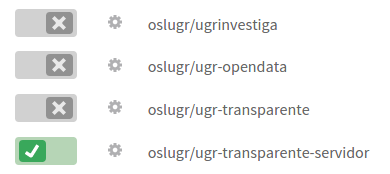
\includegraphics[width=0.5\textwidth]{../images/activar_travis.png}
		\caption{Activación de la integración continua}
		\label{fig:activar_travis}
	\end{center}
\end{figure}

La configuración por defecto de {\tt Travis} es que se compruebe la integración continua con cada \textit{``push''} o \textit{``pull request''} que se haga a nuestro repositorio, aunque esto se puede cambiar en función de nuestras preferencias.

\begin{figure}[!ht]
	\begin{center}
		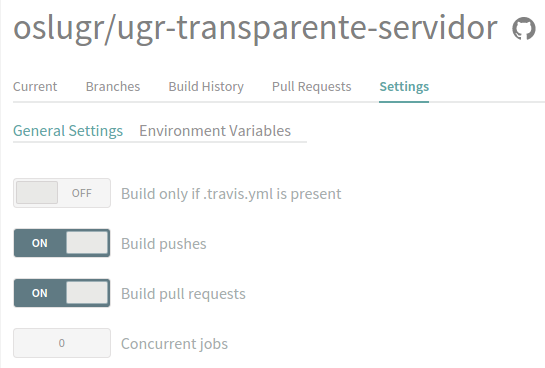
\includegraphics[width=0.6\textwidth]{../images/config_travis.png}
		\caption{Configuración de lanzamiento}
		\label{fig:config_travis}
	\end{center}
\end{figure}

Para terminar, solo nos queda crear el archivo de configuración {\tt .travis.yml} que será el que {\tt Travis} siga para comprobar la integración continua. Aspectos básicos de este archivo son indicar en {\tt language} el lenguaje en el que está escrita la aplicación y con el propio nombre del lenguaje, indicar también las versiones del mismo para las que se va a comprobar la aplicación. Para el portal hemos decidido que se comprueba la integración en las versiones estables más recientes {\tt Node.js} que son las \textit{0.10}, \textit{0.11} y \textit{0.12}, además de \textit{iojs}, que es un derivado del propio {\tt Node.js}.

\begin{lstlisting}[language=json,caption={Archivo JSON con informacion de personal},label={lst:json_personal}]
# language setting
language: node_js

# version numbers, testing against two versions of node
node_js:
- "0.12"
- "0.11"
- "0.10"
- "iojs"
\end{lstlisting}

\section{Despliegue automático}

Antes de poder realizar el despliegue automático tenemos que tener conexión mediante {\tt SSH} al servidor, además es necesario que nuestro archivo de clave pública esté copiado también el servidor. Si no tenemos un archivo de clave pública podemos generarlo con el comando ``{\tt ssh-keygen -t rsa}'', que por defecto usa un cifrado RSA de 128 bits. Ahora copiamos este archivo al servidor con el comando ``{\tt ssh-copy-id USUARIO@transparente.ugr.es}'', donde usuario es un usuario que pueda acceder mediante SSH al servidor.

\bigskip

Para realizar el despliegue tenemos que escribir un nuevo módulo con el nombre {\tt flightplan.js}. Este módulo contendrá todo el procedimiento que seguirá {\tt Flightplan} para realizar el despliegue de la aplicación en el servidor. Lo más importante a tener en cuenta en el contenido de este archivo es lo siguiente:

\begin{itemize}
	\item \textbf{plan.target}: podemos configurar el despliegue para uno o varios objetivos, por lo que tenemos que indicar un nombre para diferenciar el destino de nuestro despliegue.
	\begin{itemize}
		\item \textbf{host}: la dirección del servidor en el que vamos a desplegar la aplicación es necesario para que {\tt Flightplan} sepa dónde hacerlo.
		\newpage
		\item \textbf{username}: el usuario que ejecutará las tareas en el despliegue, hay que tener en cuenta que este usuario debe tener los permisos necesarios para ejecutar esas tareas. Por razones de seguridad/comodidad no definimos ningún usuario concreto, sino que lo introduciremos como argumento en la ejecución.
		\item \textbf{agent}: será el método que usaremos para conectarnos al servidor, en nuestro caso será una conexión {\tt SSH}.
	\end{itemize}
	\item \textbf{plan.remote}: cada una de las tareas que se ejecutarán de forma remota para realizar el despliegue se introducen en esta función.
	\begin{itemize}
		\item \textbf{remote.sudo}: estos serán los comandos que tienen que ser ejecutamos con permisos de administración.
		\item \textbf{remote.exec}: serán los comandos que se ejecutarán con el usuario que hemos lanzado el despliegue.
		\item \textbf{remote.with}: los comandos que se ejecutan en bloque después de ejecutar un comando previo.
		\item \textbf{remote.log}: estas serán las salidas que se mostrarán por pantalla y que usaremos para informar sobre el curso del proceso.
	\end{itemize}	
\end{itemize}

En el siguiente fragmento de código se puede ver como se realiza el despliegue del portal en el servidor de {\tt UGR Transparente}. Las acciones a realizar son muy simples:

\begin{itemize}
	\item \textbf{Línea 11}: realiza una copia del estado actual del portal de transparencia.
	\item \textbf{Línea 13}: sitúa el directorio actual en el directorio de la aplicación del portal.
	\item \textbf{Línea 15}: detiene la ejecución del servidor del portal.
	\item \textbf{Líneas 17 y 18}: cambia los parámetros de acceso al servidor, a los parámetros por defecto para que no se produzca un conflicto al actualizar los archivos del servidor.
	\item \textbf{Línea 20}: obtiene los nuevos cambios en la aplicación.
	\item \textbf{Línea 22}: instala las nuevas dependencias (si las hubiera).
	\item \textbf{Línea 24 y 25}: vuelve a establecer los parámetros para el acceso al servidor de forma pública.
	\item \textbf{Línea 27}: arranca el servidor para la que el portal vuelva a estar operativo.
\end{itemize}

\begin{lstlisting}[language=javascript,caption={Archivo flightplan.js},label={lst:testjs}]
var plan = require('flightplan');

plan.target('transparente', {
  host: 'transparente.ugr.es',
  username: process.env.USER,
  agent: process.env.SSH_AUTH_SOCK
});

plan.remote(function(remote) {
  remote.log('Creando copia de seguridad...');
  remote.sudo('cp -Rf ugr-transparente-servidor ugr-transparente-servidor.bak', {user: process.env.USER});

  remote.with('cd ugr-transparente-servidor',function() {
    remote.log('Deteniendo el servidor...');
    remote.exec('sudo npm run-script kill');
    remote.log('Restableciendo parametros de acceso...');
    remote.exec('sed "s/IP=transparente.ugr.es/IP=127.0.0.1/" -i package.json');
    remote.exec('sed "s/PORT=80/PORT=3000/" -i package.json');
    remote.log('Obteniendo cambios...');
    remote.exec('git pull');
    remote.log('Instalando dependencias...');
    remote.exec('sudo npm install');
    remote.log('Cambiando parametros de acceso...');
    remote.exec('sed "s/IP=127.0.0.1/IP=transparente.ugr.es/" -i package.json');
    remote.exec('sed "s/PORT=3000/PORT=80/" -i package.json');
    remote.log('Arrancando el servidor...');
    remote.exec('sudo npm start');
  });
});
\end{lstlisting}

Al finalizar el despliegue el portal estará operativo como lo estaría normalmente, hemos podido actualizarlo sin tener que acceder y aplicar la actualización manualmente. Para ejecutar el despliegue automático también se usa un script de {\tt NPM} que se ejecuta mediante ``{\tt USER=USUARIO npm run-script deploy}'', donde \textbf{USUARIO} es el usuario con acceso SSH al servidor y permisos para ejecutar todos los comandos.

\begin{lstlisting}[language=json,caption={Scripts de despliegue automático},label={lst:deploy}]
"scripts": {
  "deploy": "fly transparente"
}
\end{lstlisting}

\section{Aprovisionamiento}

\begin{lstlisting}[language=json,caption={Archivo de hosts},label={lst:hosts}]
[transparente]
transparente.ugr.es
\end{lstlisting}

\begin{lstlisting}[language=json,caption={Playbook de Ansible},label={lst:ansible}]
---
- hosts: transparente
  sudo: yes
  remote_user: "{{user}}"
  tasks:
    - name: Añadiendo repositorio para instalar Node.js...
      apt_repository: repo='ppa:chris-lea/node.js'

    - name: Actualizando lista de paquetes...
      apt: update_cache=yes

    - name: Instalando git...
      apt: name=git state=present

    - name: Instalando Node.js...
      apt: name=nodejs state=present

    - name: Clonando repositorio con la aplicacion...
      git: repo=https://github.com/oslugr/ugr-transparente-servidor.git
           dest=/home/"{{user}}"/ugr-transparente-servidor
           version=master

    - name: Cambiando propietario del directorio de la aplicacion...
      file: path=/home/"{{user}}"/ugr-transparente-servidor
            owner="{{user}}" group="{{user}}" state=directory recurse=yes

    - name: Instalando las dependencias de la aplicacion...
      npm: path=/home/"{{user}}"/ugr-transparente-servidor

    - name: Cambiando parametros de acceso (1/2)...
      command: sed "s/IP=127.0.0.1/IP=transparente.ugr.es/" -i
               /home/"{{user}}"/ugr-transparente-servidor/package.json

    - name: Cambiando parametros de acceso (2/2)...
      command: sed "s/PORT=3000/PORT=80/" -i
               /home/"{{user}}"/ugr-transparente-servidor/package.json

    - name: Arrancando el servidor...
      command: chdir=ugr-transparente-servidor npm start
\end{lstlisting}